
\documentclass[12pt]{article}
\usepackage[margin=1in]{geometry}% Change the margins here if you wish.
\setlength{\parindent}{0pt} % This is the set the indent length for new paragraphs, change if you want.
\setlength{\parskip}{5pt} % This sets the distance between paragraphs, which will be used anytime you have a blank line in your LaTeX code.
\pagenumbering{gobble}% This means the page will not be numbered. You can comment it out if you like page numbers.

%------------------------------------

% These packages allow the most of the common "mathly things"
\usepackage{amsmath,amsthm,amssymb}

% This package allows you to add images.
\usepackage{graphicx}
\usepackage{float}

% These are theorem environments.  This should cover everything you need, and you should be able to tell what environment goes with what type of result, but please let me know if I've missed anything.
\newtheorem{euclidtheorem}{Proposition}[section]
\newtheorem{classtheorem}{Theorem}
\newtheorem{theorem}{Theorem}[section]
\newtheorem{challenge}[theorem]{Challenge}
\newtheorem{question}[theorem]{Question}
\newtheorem{problem}[theorem]{Problem}


\newtheorem{theorempiece}{Theorem}[theorem]
\newtheorem{classtheorempiece}{Theorem}[classtheorem]
\newtheorem{challengepiece}{Challenge}[theorem]
\newtheorem{questionpiece}{Question}[theorem]
\newtheorem{problempiece}{Problem}[theorem]

%These help to format the names of the results the way we are in class and in notes.
\renewcommand*{\theeuclidtheorem}{\Roman{section}.\arabic{theorem}}
\renewcommand*{\thetheorem}{\arabic{section}.\arabic{theorem}}
\renewcommand*{\theclasstheorem}{\Alph{theorem}}
\renewcommand*{\thechallenge}{\arabic{section}.\arabic{theorem}}
\renewcommand*{\thequestion}{\arabic{section}.\arabic{theorem}}
\renewcommand*{\theproblem}{\arabic{section}.\arabic{theorem}}
\renewcommand*{\thetheorempiece}{\arabic{section}.\arabic{theorem}.\alph{theorempiece}}
\renewcommand*{\thechallengepiece}{\arabic{section}.\arabic{theorem}.\alph{challengepiece}}
\renewcommand*{\thequestionpiece}{\arabic{section}.\arabic{theorem}.\alph{questionpiece}}
\renewcommand*{\theproblempiece}{\arabic{section}.\arabic{theorem}.\alph{problempiece}}


% Should you need any additional packages, you can load them here. If you've looked up something (like on DeTeXify), it should specify if you need a special package.  Just copy and paste what is below, and put the package name in the { }.  
\usepackage{wasysym} %this lets me make smiley faces :-)

% Put the name of your paper here. It does not need to be a fancy name, but should tell the reader what is contained in the paper.


\title{
Predictable Pattern of Non-primes
\begin{center}
	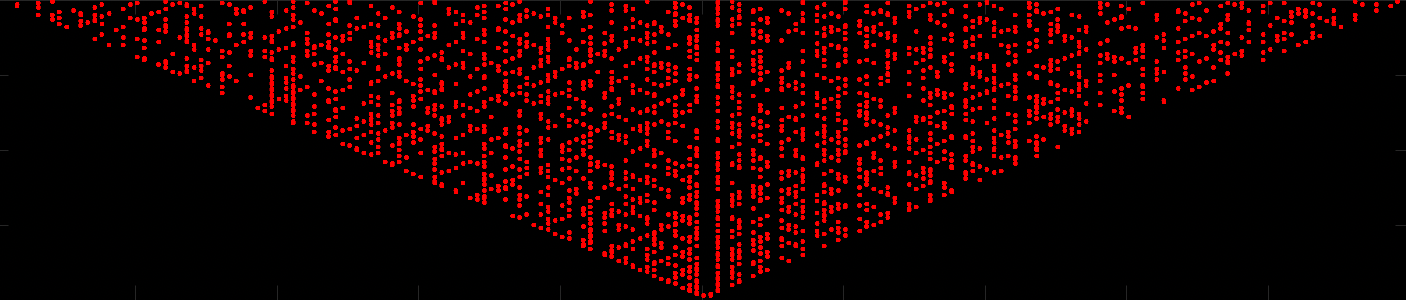
\includegraphics[width = 10cm]{titleIm.png} 
\end{center}
}
% You are the author, put your name here.
\author{Twan Mennink}

% You can change the date to be something other than the current date if you want.
\date{\today}

\begin{document}

\maketitle

This article describes an interesting pattern that reveals itself when we group the prime numbers in intervals of the form $\frac{(x-1)^2}{2} < P < \frac{x^2}{2}$ where $P$ is any prime number on the interval and x any positive integer. Furthermore a derivation of why this pattern exists is given, and implications for the prime counting function $\pi(x)$ are studied.

The results presented in this article stem from studying the patterns which are seen in prime number arrangements such as the Klauber triangle and Ulam Spiral. After experimenting with arranging the prime numbers along an Archimedes spiral with varying angular rate, a pattern started to emerge, and eventually a derivation was found that distilled the pattern to its essence, arranging primes in a triangle showing a regular vertical line pattern of no primes.

\setcounter{section}{1}
%\setcounter{theorem}{15}
%\setcounter{theorempiece}{2}

% Use the appropriate environment to get the name that you want.  
\section{Drawing the triangle}
To reveal the pattern of non-prime lines, the following must be done. Starting with $x=1$ and counting upwards, the interval from $\frac{(x-1)^2}{2}$ to $\frac{x^2}{2}$ is drawn as a horizontal line starting from right to left, centered along the origin, and vertical position equal to $x$. The length of the line segment will become
\begin{equation}
L = \frac{x^2}{2} - \frac{(x-1)^2}{2} = x - \frac{1}{2}
\end{equation}
So the centered line segment starts at $\frac{x}{2} - \frac{1}{4}$ and ends at $-\frac{x}{2} + \frac{1}{4}$.
Walking along these line sections, noting the distance traversed, a dot can be placed every time the total distance travelled is equal to a prime number. Figure \ref{firstExample} shows an example of the first ten intervals plotted as horizontal lines.
\begin{figure}[h]
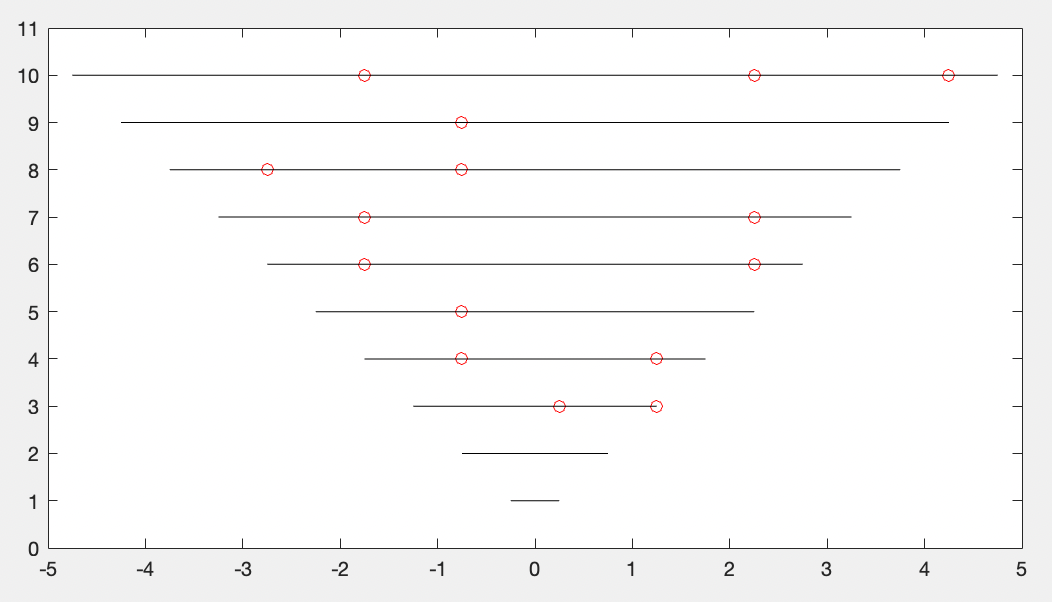
\includegraphics[width= 10cm]{primPatFirstTenLines.png}
\centering
\caption{The first ten intervals plotted horizontally}
\label{firstExample}
\end{figure}
\section{Exploring the Pattern}
The first observation is that every prime number ends up at an x-coordinate of the form $i+\frac{1}{4}$ with i an integer such that $-\frac{x}{2}+\frac{1}{4}<i+\frac{1}{4}<\frac{x}{2}-\frac{1}{4}$.
The maximal value i can take in case x is odd or x is even:
\begin{equation}
x_{odd}:	i_{max} = \frac{x}{2}-\frac{1}{2}
\label{imaxodd}
\end{equation}
\begin{equation}
x_{even}: i_{max} = \frac{x}{2}-1
\end{equation}
and the minimal value for odd x or even x:
\begin{equation}
x_{odd}:	i_{min} = -\frac{x}{2}+\frac{1}{2}
\end{equation}
\begin{equation}
x_{even}: i_{min} = -\frac{x}{2}
\end{equation}
If we want to calculate the position $p_x$ on the x-axis of a given prime number $P$, $\frac{(x-1)^2}{2} < P < \frac{x^2}{2}$, we get:
\begin{equation}
p_x = \left(\frac{x}{2}-\frac{1}{4}\right) - \left(P - \frac{(x-1)^2}{2}\right) = i+\frac{1}{4}
\end{equation}
Solving for P:
\begin{equation}
\frac{x^2}{2}-\frac{x}{2}-i = P
\label{identity1}
\end{equation}
If as an example, we take $P=11$, we can see this lies on the interval $\frac{4^2}{2}<P<\frac{5^2}{2}$, or $8<P<12.5$
If we plug this into equation \ref{identity1}, we get:
\begin{equation}
\frac{5^2}{2} - \frac{5}{2} -i = 11
\end{equation}
This results in the solution that $i=-1$.
We can think about the properties if Equation \ref{identity1}. What values of i can be a solution with prime number P. We know that $x$ is a positive integer, and $i$ is an integer. Equation \ref{identity1} is a quadratic equation, so we can factor it into two terms using the quadratic formula, and if this results in two positive integer factors, P could never have been a prime number.
\begin{align*}
&\frac{x^2}{2}-\frac{x}{2}-i = P \\\\
&a  = \frac{1}{2}, &b  = -\frac{1}{2}, &&c = -i\\\\
&x_1 = \frac{1}{2} + \sqrt{\frac{1}{4} + 2i} &=\frac{1}{2} + \frac{\sqrt{1 + 8i}}{2}\\\\
&x_2 = \frac{1}{2} - \sqrt{\frac{1}{4} + 2i} &=\frac{1}{2} - \frac{\sqrt{1 + 8i}}{2}\\\\
&a(x-x1)(x-x2)=P
\end{align*}
For example, if we use $i=1$, we get $x_1=2$ and $x_2=-1$, for this to yield two positive integers, either $(x-x_1)$ or $(x-x_2)$ must be even, so that it can be multiplied with $a$ and still be an integer.
Furtermore, for $x_1$ and $x_2$ to be integers, the identity $\sqrt{1 + 8i}$ must be odd. This only happens if $1+8i$ is an odd number squared. We can also note that only for positive $i$ there are real solutions.\par
Let $i$ be of the form:
\begin{equation}
i_k = \sum_{n=1}^{n=k}{n-1} = 0 + 1 + 2 + ... + (k-1)
\end{equation}
for every positive number $k$ this will yield a term $1 + 8i$ that is a positive odd number squared.
\begin{align*}
k=1:	&	i_1=0 & 1+8i = 1    & = 1^2\\
k=2:	&	i_2=0+1=1 & 1+8i =9& = 3^2\\
k=3:	&	i_3=0+1+2=3 & 1+8i =25& = 5^2\\
k=4:	&	i_4=0+1+2+3=6 & 1+8i =49& = 7^2\\
k=5:	&	i_5=0+1+2+3+4=10 & 1+8i =81& = 9^2
\end{align*}
Using Gauss' formula for the sum of integers, we get:
\begin{align*}
i_k &= k(k-1)/2
\end{align*}
and:
\begin{align*}
1+8i &= (2k-1)^2\\
x_1 &= \frac{1 + (2k-1)}{2} = \frac{(2k)}{2}=k\\
x_2 &= \frac{1 - (2k-1)}{2}=\frac{2 - 2k}{2}=1-k
\end{align*}
We see that whenever $k$ is even, $x_1$ will be even and $x_2$ odd, and vice versa. This means that the equation $a(x-x1)(x-x2)=P$ can always be written as two integer factors. To exclude that the position associated with this $i$ could belong to a prime number, $x$ must be larger than both $x_1$ and $x_2$, but because $x_1$ is always more positive than $x_2$, it suffices to prove that $x$ is always larger than $x_1$. There is one more condition to exclude a prime number at that location: If the term $(x-x_1)$ equals $1$, then this does not count as a factorization, so the number could still be prime.\par

**todo: implement (x-1) > 1 

We know from equation \ref{imaxodd} that $i$ is at least always smaller than:
\begin{equation*}
i < \frac{x}{2}-\frac{1}{2}
\end{equation*}
Therefore:
\begin{align*}
i_k &=k(k-1)/2 <\frac{x}{2} - \frac{1}{2}\\
&\Rightarrow k(k-1)<x-1\\
&\Rightarrow k^2-k+1<x
\end{align*}
So we know that $k^2-k+1$ is always smaller than $x$, but we want to know if $k$ is also smaller than x, because $x_1=k$. This will be true if:
\begin{align*}
k^2-k+1 &\geq k\\
\Rightarrow k^2-2k+1 &\geq 0\\
\Rightarrow (k-1)^2 &\geq 0
\end{align*}
The inequality is true for any value of k. Therefore, we can conclude that for any coordinate along the x-axis in the form of $p_x =i+\frac{1}{4}$ where $i=(k(k-1)/2$ with $k^2-k+1 < x$, we can exclude the possibility for a prime number to occupy that position.

\section{How does it look}
We can now look at how the dots for every prime number is distributed with a larger number of primes. If we take all primes under 80000, we get the result as in Figure \ref{firstExample}.
\begin{figure}[h]
\includegraphics[width= 10cm]{pattern400.png}
\centering
\caption{400 intervals plotted horizontally}
\label{SecondExample}
\end{figure}
Slightly visible there are empty vertical lines at $i=0,1,3,6,10...$. If we plot 4000 instead of 400 intervals, and zoom in, the pattern becomes very clear, as can be seen in Figure \ref{4000Example}

\begin{figure}[h]
\includegraphics[width= 17cm]{pattern3500.png}
\centering
\caption{4000 intervals plotted horizontally}
\label{4000Example}
\end{figure}
\end{document}




